\documentclass{article}

\usepackage{times}
\usepackage{uist}
\usepackage{graphicx}

\begin{document}


% --- Copyright notice ---
\conferenceinfo{UIST'09}{October 4-7, 2008, Victoria, BC, Canada}
\CopyrightYear{2009}
\crdata{x-xxxxx-xxx-x/xx/xxxx}

% Uncomment the following line to hide the copyright notice
\toappear{}
% ------------------------

\bibliographystyle{plain}

\title{HoverCross: A New Selection Paradigm for Pen-Based Interfaces}

%%
%% Note on formatting authors at different institutions, as shown below:
%% Change width arg (currently 7cm) to parbox commands as needed to
%% accommodate widest lines, taking care not to overflow the 17.8cm line width.
%% Add or delete parboxes for additional authors at different institutions. 
%% If additional authors won't fit in one row, you can add a "\\"  at the
%% end of a parbox's closing "}" to have the next parbox start a new row.
%% Be sure NOT to put any blank lines between parbox commands!
%%

\author{
\parbox[t]{9cm}{\centering
	     {\em Author Name removed for blind review}\\
	     Affiliation removed for blind review\\
         Address removed for blind review\\
	     Email removed for blind review\\}
\parbox[t]{9cm}{\centering
	     {\em Author Name removed for blind review}\\
	     Affiliation removed for blind review\\
	     Address removed for blind review\\
	     Email removed for blind review}
}

\maketitle

\abstract A central problem in pen-based interfaces is how to
transition smoothly between drawing and editing.  Separate drawing and
editing modes can be awkward and distracting, while modeless editing
gestures are error-prone.  We present HoverCross, a seamless inking and
editing interface that provides a simple and reliable method for users
to select on-screen objects.  HoverCross
combines the strengths of several recent developments in pen-based
interfaces.  With HoverCross, users ink normally and then select
objects or ink strokes by crossing over them in the hover space above
the tablet screen.  They can then edit their selection both directly and
through an editing menu.  User feedback indicates
that HoverCross provides a promising new pen-based selection technique 
that offers an efficient, fluid and predictable transition between drawing and editing.

\classification{H5.2 [Information interfaces and presentation]:
User Interfaces. - Graphical user interfaces.}

\terms{Design, Human Factors}

\keywords{Hover space, pen input, tablets.}

\tolerance=400 
  % makes some lines with lots of white space, but 	
  % tends to prevent words from sticking out in the margin

\section{INTRODUCTION}

The promise of pen-based interfaces is that they provide a natural way
for users to create diagrams and take free-form notes.  However, the
integration of diagram creation and diagram editing remains a barrier
to the widespread use of these interfaces.  Pens are more convenient
and natural for drawing, but editing with a pen remains cumbersome
when the user is forced to rely on graphical user interfaces designed
for a mouse and keyboard.  Because the user must use the pen for both
drawing and editing (or suffer the inconvenience of switching between
the pen and the keyboard), a core challenge for pen-based computing is
to construct an interface that allows users to switch easily between
the two tasks, while allowing the system to unambiguously interpret a
given pen stroke as drawing or editing.

Many people have proposed solutions to this problem in recent years.  
Traditional solutions (e.g., Windows Journal) require the user to
enter ``edit mode,'' usually by pressing a software button.  This
solution is simple, but the problems with modes are well
known~\cite{Tesler1981Smalltalk}.  Using hardware buttons to trigger mode switching
helps solve these issues because the mode switch is temporary---as
soon as the user releases the button, the interface reverts to drawing
mode.  Thus, there is little potential for mode confusion.  Studies
suggest that this approach can be quite effective and
natural~\cite{Li2005Experimental,Hinckley2006Springboard}.  However,
simply pressing the button requires not only extra physical effort,
but in many cases also an extra hand.

Other researchers take a recognition-based
approach~\cite{Saund2003Stylus,Zeleznik2008Lineogrammer}, 
attempting to distinguish
automatically between drawing and editing strokes (e.g., lasso
selections or gestures).  However, even with choice
mediators~\cite{Mankoff2000Providing} to help resolve recognition
ambiguities, recognition errors can be confusing, and gestures
can be hard to learn.  

Recently, researchers have explored using the hover space\footnote{The
\textit{hover space} is the space above the surface of a digital
tablet where the pen is still tracked but does not generate ink or
mouse events.} to invoke editing commands.  Grossman \textit{et al.}\ present
Hover Widgets~\cite{Grossman2006Hover}, in which the user performs
gestures in the hover space to activate editing menus.  Following on
this work, Subramanian \textit{et al.}\ explore the possibility of using several
layers of the hover space to perform different editing
tasks~\cite{Subramanian2006Multilayer}, while Kattinakere \textit{et
al.}\ formally model users' ability to track (e.g., execute gestures) in
hover space \cite{Kattinakere2007Modeling}.


While each of these recently developed approaches brings us closer to
the goal of seamless pen-based drawing and editing, we believe our
arsenal of drawing and editing techniques is not yet complete.  Specifically, for common diagram creation and editing tasks, Hover
Widgets or a multi-level hover space solution may be too heavyweight.

We explore the power and simplicity that can be obtained by combining
the simplest aspects of many existing techniques.  Our interface,
called HoverCross, combines the strengths of hover space editing and
crossing-based selection (e.g.,~\cite{Apitz2004Crossy}),
resulting in an interface that is straightforward to learn, reliable, and convenient
for common drawing and editing tasks.  We do not anticipate that HoverCross 
will replace all other forms of editing (e.g. gestures or temporary mode-switching).  
Rather, our approach integrates seamlessly with most other pen-based editing
techniques providing an alternative interaction style for users who prefer it.

%% Advantages of our approach: Simple, easy to learn, relatively little
%% chance of recognition error, integrates seamlessly with other
%% techniques, powerful (preferred by some users and faster than other
%% techniques for some common tasks).

%% Our interface provides
%% only one simple, reliably recognized gesture for the user to remember,
%% and this gesture is performed on the canvas so the user does not need
%% to learn to make it in hover space.  \textit{This paragraph is key and
%% needs some work.  The main contributions are that the hover space is
%% not overloaded so you don't need to use gestures in it.  Selection is
%% the number one thing you want to do in editing, and in effect it is a
%% precursor to all other editing things, so you just have to provide
%% support for that, and then you can leverage the fact that when
%% something is selected the user is probably editing.}  

%% I took this text out, but I want it around because it's nicely
%% phrased and I may have lost some of it when I wrote the text above.

%% We propose a new interface not only for creating and manipulating
%% objects with a stylus, but also for transitioning seamlessly between
%% the two tasks. Our work builds on and combines several existing
%% ideas. First, Grossman et al. explore the hover space  for diagram
%% editing [2]. We propose using this space to trigger selection reliably
%% and conveniently. To perform selection in the hover space, we use a
%% crossing metaphor, explored in CrossY, [3] as a substitute for the
%% traditional point-and-click interaction. To manipulate the selection,
%% we use a simple gesture performed on the Tablet screen to bring up a
%% ring-shaped menu around the location of the pen, as described in
%% Scriboli [4].


\section{INTERACTION USING HOVERCROSS}

In many modal pen-based interfaces (e.g., Windows Journal), it is
\textit{selection}, not editing in general, that typically
operates in its own mode.  This division makes sense, as selecting
objects in a drawing is typically the first step in performing almost
any editing task.  Once the user selects an object, she can edit it
via a menu or direct manipulation.  An explicit selection mode seems
necessary because any apparent selection stroke just as easily could
be a drawing stroke.

The key insight behind HoverCross is that relegating the process of
selection to the hover space allows users to switch between
drawing and selecting without pressing any buttons.  Furthermore,
because the user performs only selection in the hover space, a simple
crossing interface suffices, and there is no need to perform gestures
in the hover space.  The system then leverages the context of the
selection to give the user additional power through a menu or direct interaction with the selected
objects.

In our interface, the user draws normally on the screen to create
diagrams containing simple shapes and raw ink.  The Microsoft gesture 
recognition engine recognizes the shapes the
user draws, while the unrecognized ink becomes one selectable object per stroke.
Recognition is not necessary for HoverCross, but we included it in our interface so that we could explore 
using HoverCross to interact with both shapes and raw ink.

To edit the diagram, the user hovers the pen briefly over the tablet
to trigger the handles for selection and simple editing tasks (Figure~\ref{fig:handles}).  The small
vertical line that appears in the middle of the object, anchored at the bottom, is the selection handle.  
The small square and circle on the right of each object are resize and rotate handles, respectively.  
All of the handles for a shape are positioned on a faint rectangle that outlines the
shape to which they apply, to help users correlate handles to shapes.  
We discuss the functionality of each handle in more detail below.  
The brief pause before handles appear prevents triggering the handles
every time the stylus enters the range, as it inevitably does on its
way to the screen.  The length of the pause affects whether 
users accidentally trigger the handles or must wait too long.  In our tests
we found that half a second appears to work well, but we also suggest that the 
pause length be a user controlable feature.  Additionally, even if the
handles appear by mistake, the user can simply ignore them and continue to sketch.

To select an object, the user crosses the stylus in hover space over the handle in either
direction.  We chose a vertical alignment for the handles so that the crossing motion mimics the 
familiar horizontal motion of writing text.  
Once an object is selected, the rectangle surrounding the object darkens, and the handle 
realigns its anchor to the top of the shape, creating a switch-like
feel (Figure~\ref{fig:selection}).  This realignment helps prevent users from 
accidentally undoing their selection, keeps
handles from becoming too obstructive, and provides an additional visual cue to indicate 
which objects are selected.  Crossing the realigned handle in hover space (again in either direction)
deselects the shape.  As the user crosses more objects' handles, these objects
are added to the selection.  To clear the whole selection, the user moves the pen in hover
space off the edge of the screen.

The user can enter the hover space to cross one object and then immediately exit the hover space by
moving the pen tip away from the screen.  The selected object remains
selected even when the pen is outside of hover space.  To select
another object, the user simply needs to re-enter hover space near
that object.  This ability helps keep the user from accidentally selecting intervening 
objects. 

\begin{figure}[tb]
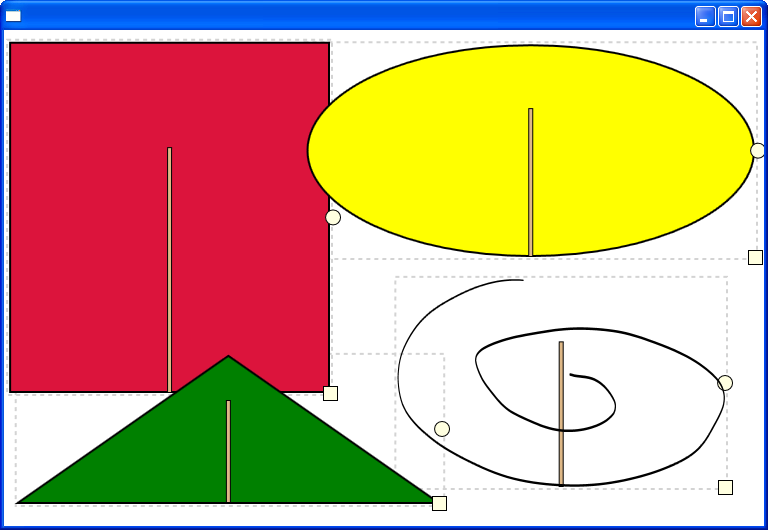
\includegraphics[width=3.0in]{SelectionHandlesOn}
\caption{Handles appear when the stylus pauses in hover space.} 
\label{fig:handles}
\end{figure}

\begin{figure}[tb]
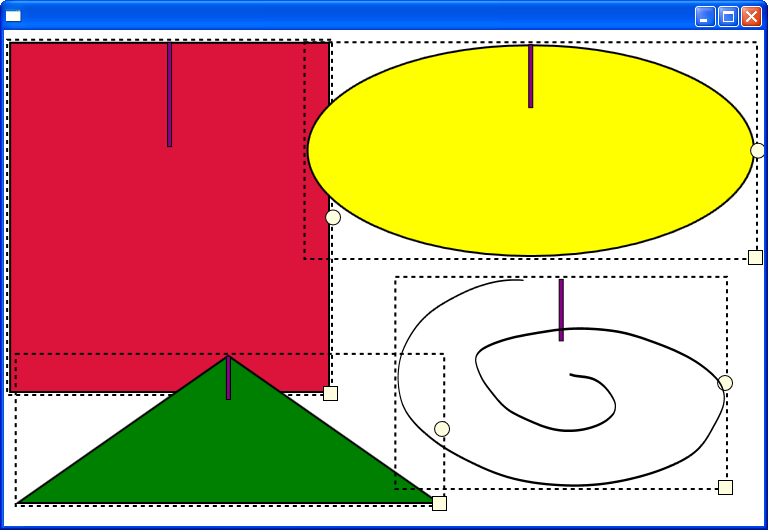
\includegraphics[width=3.0in]{SelectedObjects}
\caption{How selected objects appear.}
\label{fig:selection}
\end{figure}


Once the user has selected at least one item, she can either edit the
selected item, or continue to draw new portions of the diagram.  The
user has several options for editing the diagram.  She can move
selected shapes by dragging one of them with her pen on the
screen.  As long as she does not cross the handle in hover space,
touching the shape will not deselect it.  The user can also use the rotating and resizing handles, which we provide as
a convenience for common editing tasks.  Clicking and dragging these small shapes causes the shape to transform: the square will resize only the corresponding object, 
and the circle will rotate only the corresponding object.  
Unlike object movement, objects do not need to be selected 
to be rotated or resized, but rotating or resizing an object selects it.  
We based both of these interaction decisions on early user feedback.  

The rotate and resize handles are not unique to HoverCross; they mimic existing transformation techniques used by programs such as PowerPoint.  However, their presence demonstrates that common transformation tools do not conflict with the HoverCross paradigm.  Because selection occurs in the hover space, while transformation occurs when the pen is down, attempting to select objects will not accidentally transform them.  Because the handles are small, users are unlikely to accidentally hit them when trying to draw content, even when 
the handles are invoked by accident.


For more complicated editing tasks (e.g. copy, paste, etc), 
HoverCross can be integrated with any type of menu.  In our user studies we 
allowed editing through a context menu 
around the tip of the stylus (Figure~\ref{fig:contextMenu}), invoked either through a semicircle gesture or a 
``right-click'' gesture (i.e. pressing and holding the stylus tip to the screen).    The context menu has the advantage that with little
practice the user can easily coordinate drawing, selecting, and editing in one fluid motion.  However, designing an optimal 
menu style is tangential to our current research; HoverCross could easily be integrated with well-developed marking menus found in other
applications~\cite{Hinckley2007InkSeine,Zeleznik2008Lineogrammer}.  


\begin{figure}[tb]
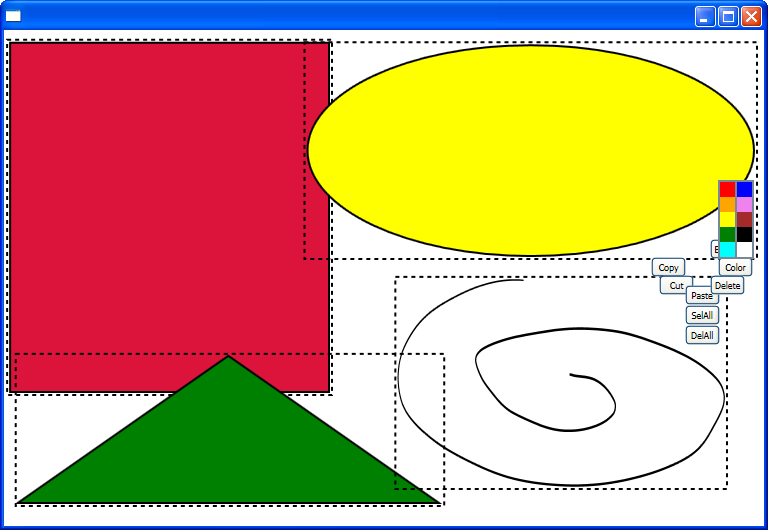
\includegraphics[width=3.0in]{ColorMenu}
\caption{The context editing menu.}
\label{fig:contextMenu}
\end{figure}

\section{DESIGN DECISIONS AND FEEDBACK}
The design of HoverCross focuses on giving users the ability to transition seamlessly between drawing and editing.  
Throughout our design we conducted several preliminary user tests to determine the effectiveness of HoverCross, and adjusted our design based on their results.  In this section we discuss 
the interface's strengths, as well as how the weaknesses we discovered through our user tests led to the final design we present above.  

%Our example application supports the creation of clean diagrams with integrated raw ink.  We chose to include 
%recognized shapes because creating polished diagrams typically requires more
%intensive editing than simply drawing freeform notes and diagrams.  In
%a previous pilot study in which we observed people creating slides in
%PowerPoint, we found that they relied heavily on copying, pasting,
%resizing and moving shapes within their diagrams.  
%However, we also included the ability to work with raw strokes
%to understand HoverCross's strengths and weaknesses for purely ink drawings.

Our user tests consisted of two phases.  In the first phase, we tested our initial design with seven users.
All users in this study were college students with some experience using a tablet computer, but no experience 
with hover or crossing-based interfaces.  
In this test, we compared three selection interfaces: our initial HoverCross design; a variation of
HoverCross called Cross; and the traditional modal lasso select.  Cross
differs from HoverCross in that users cross objects with the pen on
the screen while holding down a non-preferred hand button.  After receiving instructions and trying out the three interface techniques for about 2-5 minutes, users performed four tasks using
each of the three interface techniques.  These tasks included simple selection and editing actions, using simple, non-overlapping shapes.  We observed users and asked for their feedback.

Based on the results of our initial test we made substantial modifications to our interface, described below.  
The second phase of our user testing focused on guiding the continued modifications, and on evaluating the HoverCross's strengths and weaknesses on a more realistic, creative task.  This phase involved seven new users (again, college students with the same experience as in the first phase), but instead 
of creating and editing specific diagrams, users were told simply to draw a picture.  These pictures often became fairly complex and included shapes overlapping other shapes.  In addition, rather than testing a static interface, we refined the interface between users when we sensed we were receiving consistent feedback from users so far.  


%We confirmed several strengths about HoverCross upon implementation and after performing the users tests, including its 
%extensibility and its ability to easily work with objects lying in a row.  However, we also discovered problems associated 
%with very tall and short objects, and with objects grouped on top of each other, and took steps to mediate these problems.

\subsection{Strengths}

Our user tests consistently reflected that most users enjoyed the
transition between sketching and selecting, without the hassle of
pressing a button or other explicit indication, despite the
reliability of the button.  While some users reported that the interface
was unintuitive and hard to use at first, they also said that the interface got easier 
after a few minutes of interaction.  Users also described HoverCross as ``interesting,'' ``promising,'' and
``fun.'' 

Confirming previous results~\cite{Apitz2004Crossy}, we noticed that the crossing
selection metaphor has several advantages over traditional lasso
selection.  For selecting single shapes or shapes roughly in a
horizontal row, we observed users performing selection quickly and reliably.  Some users
commented that for small selections drawing
a circle around the objects seemed excessive, and they preferred the crossing metaphor.  
Additionally, when selecting shapes spread out in space, users generally had no trouble 
learning to enter and exit hover space to avoiding selecting
intervening objects.  Users reported that they felt that selecting a few
spatially separated objects with lasso
select was awkward, while with HoverCross they could simply move the
pen across the screen to the objects of interest.  

A final strength of this interface is that any part of it may be
implemented in conjunction with most other pen-based interface techniques.  
Because the hover selection interface requires a short pause to invoke, the
user is not likely to trigger it by mistake, so it may be combined
with a traditional modal selection interface.  For example, a user
might use modal lasso selection to select a group of tightly clumped
objects, and then use HoverCross to deselect one of them.


\subsection{Design Modifications in Response to Common Problems}

\subsubsection{Handle placement.}  
A common problem we discovered in the first user tests was that if handles are the same height as their shapes, they would either be too easily selected or too difficult to select if the shapes were either too tall or too short.  So, rather than having the selection handles fit the shapes precisely, we gave the handles minimum and maximum sizes.  We also made the handles switches that change position and color depending on whether their shape is selected to facilitate user interaction, so the handles could never extend across the entire shape.  Users in latter tests approved of the switch paradigm, and frequently commented that although it took some time to get used to, object selection became natural and fit well with the drawing system.

\subsubsection{Occluded Shapes}
Another common problem we found in early user tests was the fact that shapes obstructed by other shapes would be either difficult or impossible to select.  We fixed this problem by counting crosses over obstructed handles as legitimate crosses.  This improvement consistently tested well when given to users for feedback.  Although we worried that allowing crossing selection of obstructed shapes might produce accidental selections, users rarely cited it as a problem, in contrast with the negative feedback we received about the inability to select obstructed shapes.

Still, this improvement gave rise to another complication in the user tests, when shapes were grouped directly on top of other shapes.  For example, if one handle became grouped directly on top of another handle, the user would switch them both simultaneously.  Although annoying, this was never a critical flaw, because users could simply resort to another means of selection, such as tapping the rotation circle and moving the shape on top.  It is also worth noting that lasso selection does not solve this problem, either, since lassoing would always select both shapes as well.  Indeed, HoverCross is probably an improvement in precision over lasso selection for cluttered diagrams, since the selection process is precise to a single, visible line segment.

\subsubsection{Resizing and Rotating} Our initial prototype did not allow users to resize or rotate objects.  We quickly realized that these abilities were important to enable more realistic interaction with the system.  
We added the rotation and resize handles as described above, and users' responses were overwhelmingly positive.  The only change we made to these handles based on user feedback was to allow users to rotate and resize an object without having 
to select the object first.


\subsection{Future Improvements}

Despite HoverCross's promise, there are several improvements we would like to explore.  
First, users occasionally complained about the selection boxes becoming too cluttered, particularly for diagrams with many small strokes; we could address this problem by grouping strokes or by changing the selection box paradigm for strokes, for example having the box fit the stroke more tightly.  Second, most users found HoverCross cumbersome for selecting a large number of tightly grouped objects, where a lasso or box-select seemed more appropriate.  As mentioned above, we could address this problem by integrating HoverCross with traditional lasso select, or perhaps by introducing a box or lasso-select ability directly in the hover space.  Third, a number of user's comments focused on difficulties with the shape recognizer or invoking the context menu.  These aspects are not central to the HoverCross paradigm, but improving them would allow users to focus solely on the utility of HoverCross.  

%Finally, although we claim that HoverCross can be combined with other interaction techniques, we must actually perform and %test this integration to understand how well this integration works in practice.  

%Our first preliminary user test involved four tasks.  We collected qualitative data on which interface users preferred for %each task.  For these same tasks, four users preferred HoverCross over the other
%two interfaces (Figure~\ref{tab:pref}).  Only in task 2, which involved selecting a group of closely placed objects, did 
%users tend to prefer lasso select to crossing.  This result is
%understandable, because crossing over each individual object in the
%group is more cumbersome than drawing a lasso around it.  However, one
%user still preferred HoverCross for this task.  He reflected that,
%while both interfaces are effective, HoverCross was more interesting
%and fun.


%\begin{figure}
%\begin{center}
%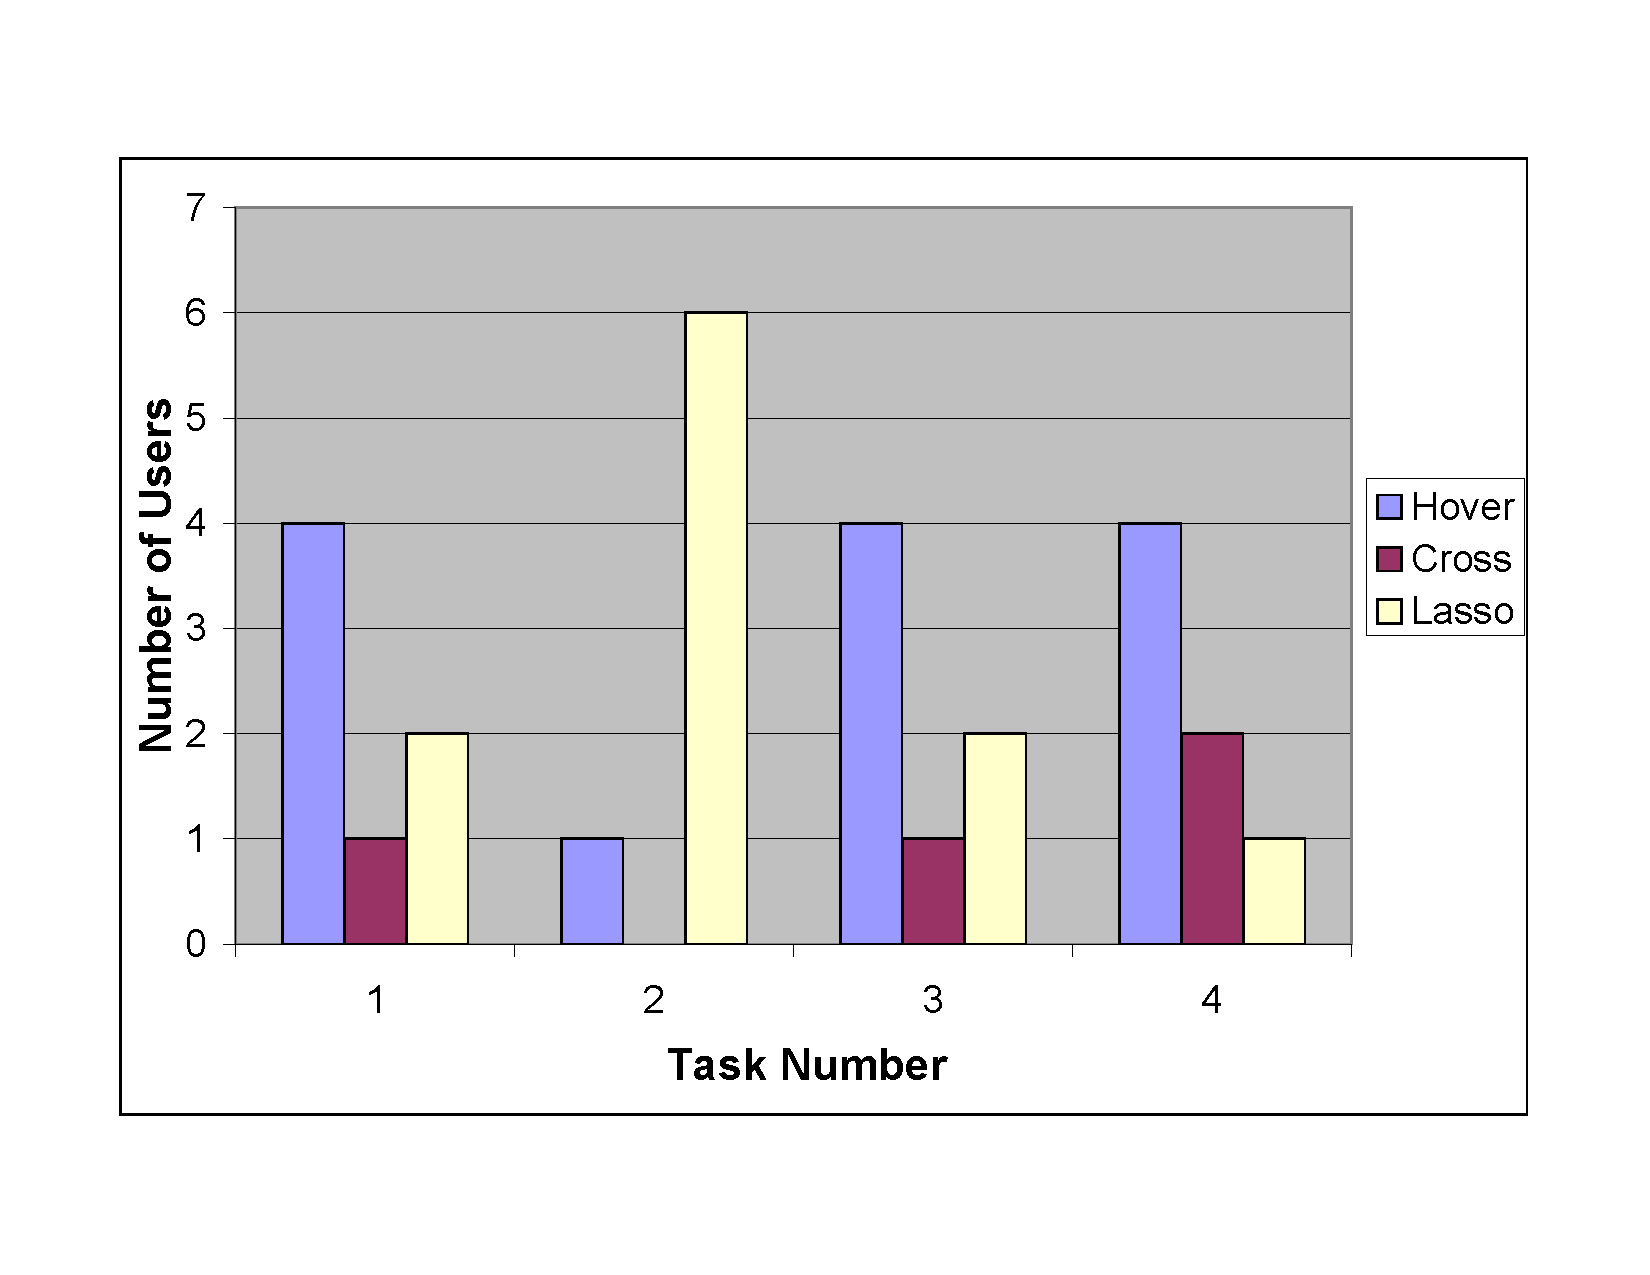
\includegraphics[width=3.0in]{Preferences}
%\caption{Number of users who preferred each interface for each task.}
%\label{tab:pref}
%\end{center}
%\end{figure}



\section{IMPLEMENTATION}

This interface, designed for the Tablet PC, is written in C\# using
Windows Presentation Foundation and .NET 3.0.  We use the built-in
gesture and text recognizers.  We recognize movement in the hover
space by handling the StylusInAirMove event, tracking the stylus
position, and selecting or deselecting an object whenever the stylus
crosses its handle.

HoverCross determines whether or not a motion crosses a handle by storing the previous stylus location and passing it, along with the current stylus location, to an intersection test.  This test checks whether the line segment between the two points crosses the center of any handles.  If it does, the method returns all the handles that the motion crosses.

%Our context menu is a
%collection of Button UIElements stored on the InkCanvas, each
%representing an editing option.  When the user clicks on any of the
%buttons, the system performs the desired option on all selected items.

\section{CONCLUSION}
HoverCross combines many simple and effective ideas from
recent advances in pen-based interfaces to provide an integrated
interface for inking and editing.  Used in combination with other
pen-based interaction techniques, we believe HoverCross will bring us one step
closer to the goal of creating pen-based interfaces that combine the
freedom of paper with the power of the computer in a useful, and
usable, way.  

% use \newpage to break the columns on the last page so they have equal length
% if the break occurs in the middle of a paragraph, insert \linebreak before \newpage
%\linebreak
%\newpage

\section{ACKNOWLEDGEMENTS}
Removed for blind review.
%We would like to thank our users who helped us evaluate HoverCross.  Much of this work was funded by the Baker Foundation %and an NSF CAREER award
%(IIS-0546809).

%%%	You can use bibtex if you like, but I've hardwired in these 
%%%	references to avoid sending you a separate .bib file.
\bibliography{uist08}



\end{document}
